\documentclass[]{beamer}
\usepackage[T1]{fontenc}
\usepackage[utf8]{inputenc}
\usepackage{lmodern}
\usepackage[italian]{babel}
\usepackage{mathrsfs}
\usepackage{cancel}

\title{La dinamica}
\author{\texorpdfstring{Mattia Cozzi\newline\href{mailto:cozzimattia@gmail.com}{\texttt{cozzimattia@gmail.com}}}{Mattia Cozzi}}
\date{a.s.~2023/2024}

%\documentclass[handout]{beamer}     %usare questa classe per generare l'handout
%\usepackage{pgfpages}   %per mostrare più quadri nella stessa pagina
%\pgfpagesuselayout{4 on 1}[a4paper,border shrink=5mm,landscape]
\usetheme{Singapore}
%\useoutertheme[left]{sidebar} %elementi intorno alle diapositive
\setbeamercovered{dynamic} %modifica l'aspetto del testo grigetto delle diapositive future. Argomenti: invisible/transparent/dynamic
\usecolortheme{orchid}
%COLORE PRINCIPALE
\definecolor{marroncino}{RGB}{156, 26, 0} % UBC Blue (primary)
\setbeamercolor{structure}{fg=marroncino} % itemize, enumerate, etc

\theoremstyle{plain}
\newtheorem{teorema}{Teorema}

\usepackage{tikz}
\usepackage{circuitikz}

\usepackage{pgf,pgfplots,graphicx}
\usetikzlibrary{angles,quotes,arrows,shapes,decorations.markings}
\pgfplotsset{compat=1.15}
\usepgfplotslibrary{units,fillbetween} % to add units easily to axis

\newcommand{\fem}{f_{em}}

\def\angolo[#1](#2)(#3:#4:#5)% Syntax: [draw options] (center) (initial angle:final angle:radius)
    { \draw[#1] ($(#2)+({#5*cos(#3)},{#5*sin(#3)})$) arc (#3:#4:#5); }


\begin{document}

\begin{frame}
  \titlepage
\end{frame}





\begin{frame}
\frametitle{Contenuti}
\tableofcontents
\end{frame}








\section{Dinamica}


\begin{frame}
\frametitle{Contesto storico}
\begin{columns}
\begin{column}{0.2\textwidth}
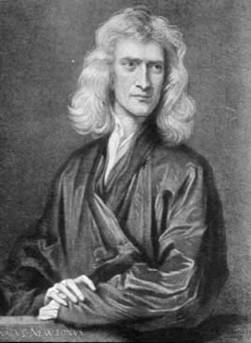
\includegraphics[width=\columnwidth]{img/newton.jpg}
\end{column}
\begin{column}{0.7\textwidth}
1687\\\emph{Philosophiae Naturalis Principia Mathematica}\pause

\begin{itemize}
\item teoria eliocentrica di Copernico (1543);\pause
\item leggi di Keplero (1609);\pause
\item legge di inerzia di Galileo (1632).\pause
\end{itemize}
Concetto centrale dell'opera di Newton è quello di \alert{forza} (in greco $ \delta \upsilon \nu \alpha \mu \iota \varsigma $, \emph{dynamis}).
\end{column}
\end{columns}
\end{frame}



\begin{frame}
  \frametitle{Strumento di misura}
    Le forze possono essere misurate mediante un \emph{dinamometro}:
  \begin{columns}
    \begin{column}{0.45\textwidth}
      \begin{figure}
        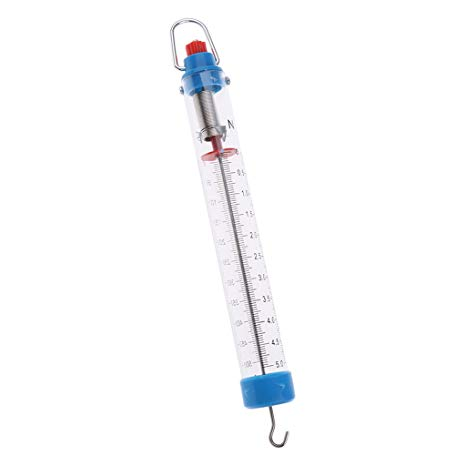
\includegraphics[width=\columnwidth]{img/dinamometro1.jpg}
        
        Dinamometro analogico
      \end{figure}
      
    \end{column}
    \begin{column}{0.45\textwidth}
      \visible<2>{\begin{figure}
        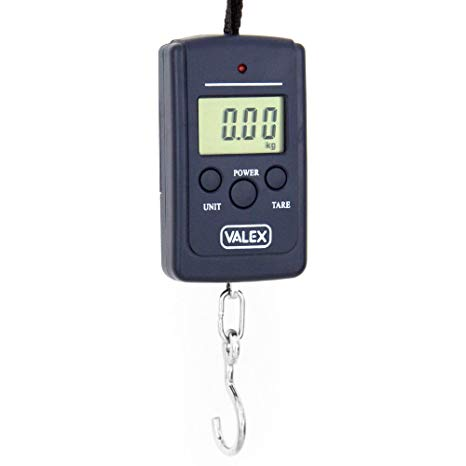
\includegraphics[width=\columnwidth]{img/dinamometro2.jpg}
        Dinamometro digitale
      \end{figure}
      }
    \end{column}
  \end{columns}
\end{frame}





\section{Primo}




\begin{frame}
  \frametitle{Enunciato del primo principio}
\begin{block}{Principio d'inerzia}
Un punto materiale mantiene costante la propria velocità se e solo se è soggetto a una forza totale nulla.
\begin{center}
\colorbox{marroncino!30}{$ \vec{v} = cost \Longleftrightarrow \sum \vec{F} = 0 $}\pause
\end{center}
In particolare, quando la velocità è nulla il corpo è inizialmente fermo e continua a rimanere fermo.
\end{block}
\end{frame}


\begin{frame}
\frametitle{Esempio}
\begin{exampleblock}{Mantenere la velocità}
{\small Un'auto viaggia alla velocità costante di $ 75 \, \frac{km}{h} $. Quanto valgono le forze frenanti (attrito con l'aria, con la strada, ecc.) se il motore spinge con una forza di $ 732 \, N $?}
\end{exampleblock}
\end{frame}




\begin{frame}
  \frametitle{Galileo}
\begin{block}{Sistema di riferimento inerziale}
I sistemi di riferimento inerziali sono sistemi di riferimento in cui vale il principio di inerzia.
\end{block}\pause
\begin{block}{Principio di relatività galileiana}
Le leggi della meccanica sono le stesse in tutti i sistemi di riferimento inerziali.
\end{block}\pause
\begin{alertblock}{Stiamo ``semplificando''!}
La relatività galileiana ha come ambito di applicazione velocità molto minori di quella luce nel vuoto, $ c = 3,0 \times 10^8 \, \frac{m}{s} $.
\end{alertblock}
\end{frame}

\begin{frame}
  \frametitle{Nelle parole di Galileo}
  \begin{quote}
    Rinserratevi con qualche amico nella maggiore stanza che sia sotto coverta di alcun gran navilio, e quivi fate d’aver mosche, farfalle e simili animaletti volanti; siavi anco un gran vaso d’acqua, e dentrovi de’ pescetti; sospendasi anco in alto qualche secchiello, che a goccia a goccia vada versando dell’acqua in un altro vaso di angusta bocca [\ldots]. Osservate che avrete diligentemente tutte queste cose, benché niun dubbio ci sia che mentre il vassello sta fermo non debbano succeder così, fate muover la nave con quanta si voglia velocità; ché (pur che il moto sia uniforme e non fluttuante in qua e in là) voi non riconoscerete una minima mutazione in tutti li nominati effetti, né da alcuno di quelli potrete comprender se la nave cammina o pure sta ferma.
  \end{quote}
\end{frame}


\section{Secondo}


\begin{frame}
\frametitle{Massa inerziale}
La medesima forza applicata ad un triciclo o ad un'automobile produce effetti diversi.\pause

~

Chiamiamo la proprietà che permette agli oggetti di resistere ad un'accelerazione \alert{massa inerziale} e la misuriamo in $ kg $.\pause

~

Una massa più grande sarà più difficile da accelerare rispetto ad una massa minore.
\end{frame}


\begin{frame}
  \frametitle{Enunciato del secondo principio}
\begin{block}{Legge fondamentale della dinamica}
L'accelerazione di un corpo è direttamente proporzionale alla forza agente su di esso, mentre è inversamente proporzionale alla sua massa inerziale.\pause
\begin{center}
\colorbox{marroncino!30}{$ \vec{F} = m \vec{a} $}
\end{center}
\end{block}
\pause
Una forza agente su un corpo causerà un'accelerazione nel corpo, ovvero una \alert<3>{variazione del vettore velocità} del corpo.
\end{frame}


\begin{frame}
  \frametitle{Unità di misura della forza}
  A partire dal secondo principio: \[ \textcolor{orange}{\vec{F}} = \textcolor{cyan}{m}  \textcolor{magenta}{\vec{a}}  \]
  definiamo l'unità di misura della forza, il \emph{newton}:
  \[ 1 \, \textcolor{orange}{N} = 1 \, \textcolor{cyan}{kg} \cdot \textcolor{magenta}{\frac{m}{s^2}} \]
\end{frame}


\begin{frame}
\frametitle{Esempio}
\begin{exampleblock}{Moto su un piano}
{\small Non conosciamo la massa di una scatola appoggiata su un piano senza attrito, ma sappiamo che se la spingiamo per $ 2,0 \, s $ con una forza costante di $ 2,0 \, N $ essa acquista una velocità di $ 15 \, \frac{m}{s} $. 

\begin{itemize}
  \item Qual è la massa della scatola?
\end{itemize}}
\end{exampleblock}
\end{frame}



\begin{frame}
  \frametitle{Un caso particolare}
\begin{block}{Forza peso}
Forza che un pianeta esercita sui corpi posti in prossimità della sua superficie.\pause
\begin{center}
\colorbox{marroncino!30}{$ \vec{P} = m \vec{g} $}
\end{center}\pause
Il valore dell'accelerazione di gravità (detta anche ``intensità del campo gravitazionale'') $ \vec{g} $ dipende dal pianeta. Sulla Terra, $ g_T = 9,81 \, \frac{m}{s^2} $, su Marte, $ g_M = 3,71 \, \frac{m}{s^2} $.
\end{block}\pause
\begin{alertblock}{Osservazione importante}
  Il modulo di $ \vec{g} $ non dipende dalla massa del corpo: nel vuoto, tutti i corpi cadono con la medesima accelerazione! \href{video/Piumapalla.mp4}{\beamergotobutton{Video: Piuma e palla}}
\end{alertblock}
\end{frame}





\section{Terzo}

\begin{frame}
  \frametitle{Enunciato del terzo principio}
\begin{block}{Principio di azione e reazione}
Se un corpo A agisce con una forza su un corpo B, anche B esercita una forza sul corpo A: le due forze hanno lo stesso modulo, stessa direzione e versi opposti.\pause
\begin{center}
\colorbox{marroncino!30}{$ \vec{F}_{A \rightarrow B} = - \vec{F}_{B \rightarrow A} $}
\end{center}
\end{block}
\end{frame}


\begin{frame}
\frametitle{Esempio}
\begin{exampleblock}{Spinta reciproca}
{\small Una pattinatrice di $ 50 \, kg $ spinge un suo compagno di $ 70 \, kg $ ed acquista un'accelerazione di $ 1,3 \, \frac{m}{s^2} $.

\begin{itemize}
  \item Qual è l'accelerazione del secondo pattinatore?
\end{itemize}}
\end{exampleblock}
\end{frame}



\section{Forze}

\begin{frame}
  \frametitle{Peso}
\begin{block}{Forza peso}
Forza che un pianeta esercita sui corpi posti in prossimità della sua superficie.\pause
\begin{center}
\colorbox{marroncino!30}{$ \vec{P} = m \vec{g} $}
\end{center}
\end{block}\pause
È sempre diretta ``verso il basso'', cioè verso il centro del pianeta, ed è pertanto una forza \alert{centripeta} (da \emph{centrum}, centro + \emph{petere}, andare).
\end{frame}



\begin{frame}
\frametitle{Attrito}  
\begin{block}{Forza d'attrito}
Forza di contatto che si oppone al moto di scivolamento o rotolamento di un corpo su una superficie.\\~\\\pause
\begin{center}
\colorbox{marroncino!30}{$ F_{As} \leq \mu F_\perp $}
\end{center}
\end{block}\pause
Notiamo che l'attrito è direttamente proporzionale all'intensità della \alert{forza premente} $ F_\perp $.
\end{frame}

\begin{frame}
\frametitle{Esempi}
\begin{exampleblock}{Spingere una cassa}
\begin{small}
Calcola la forza orizzontale necessaria a spostare una cassa di $ 1,28 \, kg $ su un piano con coefficiente d'attrito statico $ \mu = 0,43 $.
\end{small}
\end{exampleblock}

~

\begin{exampleblock}{La forza è sufficiente?}
\begin{small}
Una forza orizzontale di $ 23,0 \, N $ è sufficiente per spostare una cassa di $ 8,00 \, kg $ su un piano con coefficiente di attrito statico $ \mu = 0,330 $?
\begin{itemize}
  \item Qual è la massima massa spostabile?
\end{itemize}
\end{small}
\end{exampleblock}
\end{frame}


\begin{frame}
  \frametitle{Richiamo}
\begin{block}{Forza elastica}
Forza direttamente proporzionale allo spostamento di un corpo con proprietà elastiche (come una molla).

\begin{center}
\colorbox{marroncino!30}{$ \vec{F} = - k \Delta \vec{x} $}
\end{center}
$ k = $ costante elastica della molla $ \left[ \dfrac{N}{m} \right]$

~

$ \Delta \vec{x} = $ spostamento della molla dalla posizione di equilibrio $ [m] $
\end{block}\pause

~

Tale forza tende a riportare il corpo nella posizionale iniziale, ed è pertanto una \alert{forza di richiamo}.
%grafico della proporzionalità diretta
\end{frame}

\begin{frame}
\frametitle{Esempio}
\begin{exampleblock}{Rimbalzo}
{\small Immagina di poter rendere un trampolino elastico come una molla con costante elastica $ k = 1200 \, \frac{N}{m} $.
\begin{itemize}
  \item Quanto è compresso quando un saltatore di $ 70,0 \, kg $ inizia la sua risalita durante un rimbalzo?
\end{itemize}
}
\end{exampleblock}
\end{frame}

\begin{frame}
\frametitle{Reazione normale/vincolare}
Quando appoggiamo un oggetto su un tavolo, il tavolo sostiene l'oggetto esercitando libro una forza perpendicolare/normale alla sua superficie detta \alert{reazione vincolare $ \vec{N} $}.\pause

~

In generale, una superficie esercita una reazione vincolare \alert{sempre perpendicolarmente} a sé stessa.


\begin{columns}
\begin{column}{0.45\textwidth}
\begin{figure}
\begin{tikzpicture}[scale=.5]
%il piano e la scatola
\draw [] (1,0) -- (6,0);
\draw [fill=brown!50] (3,0) -- (3,1) -- (4,1) -- (4,0) -- (3,0);

%la forza peso
\draw [->,blue!40,ultra thick] (3.5,.5) -- (3.5,-2);
\node [left,blue!40] at (3.5,-1) {{\scriptsize $ \vec{P} = m\vec{g} $}};

%reazione normale
\draw [->,ultra thick,red!70] (3.5,.5) -- (3.5,3);
\node [left,red!70] at (3.3,2) {{\scriptsize $ \vec{N} $}};

%centro di massa
\draw [fill, ultra thick] (3.5,.5) circle [radius=.02];
\end{tikzpicture}
\end{figure}
\end{column}
\begin{column}{0.45\textwidth}
\begin{figure}
\begin{tikzpicture}[scale=.5]
%il piano e la scatola
\draw [] (0,5) -- (6,1.25);
\draw [fill=brown!50] (2,3.75) -- (2.53,4.6) -- (3.53,3.97) -- (3,3.13) -- (2,3.75);

%la forza peso
\draw [->,blue!40,ultra thick] (2.76,3.86) -- (2.76,1);
\node [left,blue!40] at (2.7,2.3) {{\scriptsize $ \vec{P} = m\vec{g} $}};

%reazione normale
\draw [->,ultra thick,red!70] (2.76,3.86) -- (4.05,5.92);
\node [above left,red!70] at (3.67,5.15) {{\scriptsize $ \vec{N} $}};

%centro di massa
\draw [fill, ultra thick] (2.76,3.86) circle [radius=.02];
\end{tikzpicture}
\end{figure}
\end{column}
\end{columns}


\end{frame}


\section{Equilibrio}



\begin{frame}
  \frametitle{Equilibrio di un punto materiale}
\begin{block}{Condizione di equilibrio di un punto materiale ($ a=0 $)}
Affinché un corpo \emph{rimanga fermo} o \emph{si muova di moto uniforme}, è necessario che:
\begin{center}
\colorbox{marroncino!30}{$ \sum \vec{F} = 0 $}
\end{center}\pause
\end{block}
Le forze sono delle \alert{quantità vettoriali}, e quando eseguiamo calcoli su di esse dobbiamo ricorrere al calcolo vettoriale.
\end{frame}





\begin{frame}
\frametitle{Corpi estesi}
Non tutti i corpi possono essere efficacemente rappresentati come dei punti.\pause

~

La \alert{dinamica dei corpi estesi} (corpi rigidi) deve prendere in considerazione:
\begin{itemize}
  \item le forze applicate ad un corpo;
  \item il punto di applicazione della forza;
  \item l'angolo di applicazione.
\end{itemize}
\end{frame}



\section{Momento}

\begin{frame}
\frametitle{Rotazioni}
Utilizzeremo:
\begin{itemize}
  \item la \alert<1>{forza $ \vec{F} $}, applicata in un certo punto dell'oggetto;\pause
  \item il \alert<2>{punto $ O $}, scelto a piacimento (spesso è il centro della rotazione dell'oggetto);\pause
  \item il \alert<3>{vettore $ \vec{r} $} (braccio della forza), che collega $ O $ al punto di applicazione della forza.
\end{itemize}
\begin{figure}
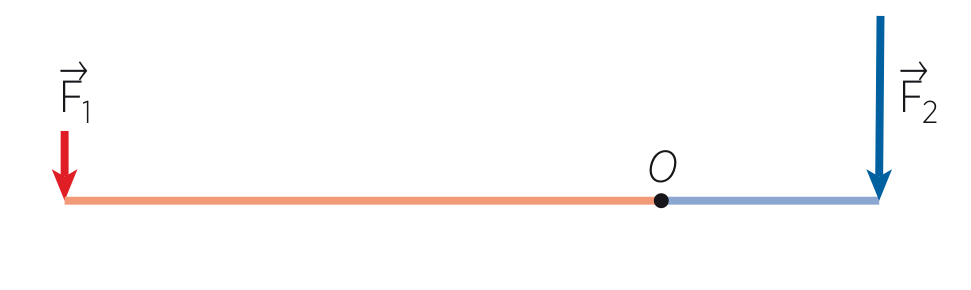
\includegraphics[width=.5\columnwidth]{img/braccioforza.png}
\end{figure}
\end{frame}


\begin{frame}
\frametitle{Momento di una forza (momento torcente)}
\begin{block}{Momento di una forza}
Il momento (torcente) $ M $ della forza $ \vec{F} $ applicata con un angolo $ \theta $ rispetto al punto $ O $ è dato da:
\begin{center}
\colorbox{marroncino!30}{$ M=rF\sin\theta $}
\end{center}

\end{block}
\end{frame}


\begin{frame}
\frametitle{Il ruolo dell'angolo}

\begin{columns}
\begin{column}{0.3\textwidth}
\begin{figure}
\begin{tikzpicture}[scale=.5,rotate=0]
\angolo[black](1.5,-.5)(0:90:.8)
\node [left,thick] at (2.2,.6) {{\tiny $ \theta $}};
\node [left,blue,thick] at (1.5,1) {{\tiny $ \vec{F} $}};
\draw [->,blue,thick] (1.5,-.5) -- (1.5,2);
\node [left,red,thick] at (3.5,0) {{\tiny $ \vec{r} $}};
\draw [<-,red,thick] (1.5,-.5) -- (3,-.5);
\end{tikzpicture}

~

{\footnotesize $ \sin\theta = 1 $\\momento massimo

~

forza efficace}
\end{figure}
\end{column}
\begin{column}{0.3\textwidth}
\vspace{.82cm}
\begin{figure}
\begin{tikzpicture}[scale=.5,rotate=270]
\angolo[black](1.5,-.5)(270:90:.8)
\node [above,thick] at (.8,-.5) {{\tiny $ \theta $}};
\node [above,blue,thick] at (1.5,1.5) {{\tiny $ \vec{F} $}};
\draw [->,blue,thick] (1.5,-.5) -- (1.5,2.5);
\node [below,red,thick] at (1.5,-1.5) {{\tiny $ \vec{r} $}};
\draw [<-,red,thick] (1.5,-.5) -- (1.5,-2.5);
\end{tikzpicture}

{\footnotesize $ \sin\theta = 0 $\\momento nullo

~

forza inefficace}
\end{figure}



\end{column}
\begin{column}{0.3\textwidth}
\vspace{1.29cm}
\begin{figure}
\begin{tikzpicture}[scale=.5,rotate=307]
\angolo[black](1.5,-.5)(52:90:.8)
\node [above left,thick] at (2.3,.6) {{\tiny $ \theta $}};
\node [left,blue,thick] at (1.4,1.2) {{\tiny $ \vec{F} $}};
\draw [->,blue,thick] (1.5,-.5) -- (1.5,2);
\node [above,red,thick] at (3.5,.8) {{\tiny $ \vec{r} $}};
\draw [<-,red,thick] (1.5,-.5) -- (3,1.5);
\end{tikzpicture}

{\footnotesize $ 0 < \sin\theta < 1 $\\momento ``intermedio''

~

forza parzialmente efficace}
\end{figure}
\end{column}
\end{columns}
\end{frame}



\begin{frame}
\frametitle{Equilibrio di un corpo rigido}
\begin{block}{Condizione di equilibrio di un corpo rigido}
Affinché un corpo esteso \emph{rimanga in equilibrio} è necessario che:
\[ \left\{ 
  \begin{array}{l}
  \sum \vec{F} = 0\\
  \,\\
  \sum \vec{M} = 0
  \end{array}
  \right.  \]
\end{block}
\end{frame}

\begin{frame}
\frametitle{Esempio}
\begin{exampleblock}{Altalena}
{\small Un'altalena ha i bracci asimettrici, uno da $ 2,5 \, m $ e uno da $ 2,0 \, m $.
\begin{itemize}
  \item Quale forza dobbiamo esercitare sul braccio da $ 2,0 \, m $ per equilibrare il peso di un bambino di massa $ 25,0 \, kg $?
  \item Quale forza esercita il sostegno dell'altalena?
\end{itemize}}
\end{exampleblock}
\end{frame}



\end{document}
